\documentclass[tikz]{standalone}
\tikzset{% define pic styles
  pics/array/.style={
   code=
   {
    \draw(-0.6,0)--+(1.2,0);
    \draw(0,-0.6)--+(0,1.2);
    \draw[fill=red!50] circle[red!50,radius=4pt](0,0);
    \foreach \a in {0.5,-0.5} {
      \draw[fill=green!50] (0,\a) circle[radius=2pt];
      \draw[fill=green!50] (\a,0) circle[radius=2pt];
    }
    }
  }
}

\begin{document}
  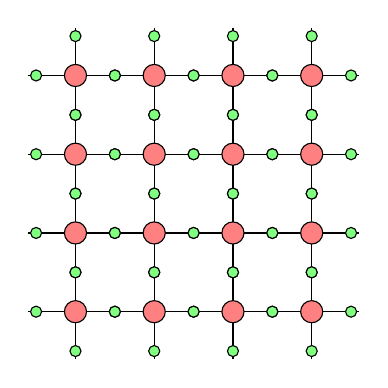
\begin{tikzpicture}
    \foreach \x in {0, ..., 3} {
      \foreach \y in {0, ..., 3} {
      
        \draw (\x, \y) pic{array};
      }
    }
  \end{tikzpicture}
\end{document}
